\documentclass{article}
% if you need to pass options to natbib, use, e.g.:
\PassOptionsToPackage{numbers, compress}{natbib}
% before loading neurips_2023
\usepackage[final]{neurips}
% to avoid loading the natbib package, add option nonatbib:
%    \usepackage[nonatbib]{neurips}


\usepackage[utf8]{inputenc} % allow utf-8 input
\usepackage[T1]{fontenc}    % use 8-bit T1 fonts
\usepackage{hyperref}       % hyperlinks
\usepackage{url}            % simple URL typesetting
\usepackage{booktabs}       % professional-quality tables
\usepackage{amsmath}        % extended math commands such as \operatorname and \eqref
\usepackage{amsfonts}       % blackboard math symbols
\usepackage{nicefrac}       % compact symbols for 1/2, etc.
\usepackage{microtype}      % microtypography
\usepackage{xcolor}         % colors
\usepackage{graphicx}
\usepackage{tikz}
\usetikzlibrary{arrows.meta}


\title{BirdGEN: Conditional Spectrogram Augmentation for Bird Species Classification under Simulated Label Scarcity}


% The \author macro works with any number of authors. There are two commands
% used to separate the names and addresses of multiple authors: \And and \AND.
%
% Using \And between authors leaves it to LaTeX to determine where to break the
% lines. Using \AND forces a line break at that point. So, if LaTeX puts 3 of 4
% authors names on the first line, and the last on the second line, try using
% \AND instead of \And before the third author name.


\author{%
  \begin{tabular}[t]{@{}c@{\hspace{0.8em}}c@{\hspace{0.8em}}c@{}}
    Shenghao Jin & Harvey Li & Vincent Wang \\
    {\normalfont\small Department of Electrical and} &
    {\normalfont\small Department of Electrical and} &
    {\normalfont\small Department of Electrical and} \\
    {\normalfont\small Computer Engineering} &
    {\normalfont\small Computer Engineering} &
    {\normalfont\small Computer Engineering} \\
    {\normalfont\small University of Toronto} &
    {\normalfont\small University of Toronto} &
    {\normalfont\small University of Toronto} \\
    {\scriptsize\texttt{shenghao.jin@mail.utoronto.ca}} &
    {\scriptsize\texttt{harv.li@mail.utoronto.ca}} &
    {\scriptsize\texttt{vz.wang@mail.utoronto.ca}} \\
  \end{tabular}
}

\begin{document}


\maketitle

\begin{abstract}
BirdGEN investigates whether class-conditional spectrogram generation can
improve bird-species classification when labeled data are limited.  We use
recording-isolated log-mel preprocessing, Residual CNN and CRNN classifiers,
and a progressively refined conditional VAE.  The downstream study preserves
nine matched blocks and the four per-species conditions $50+0$, $50+50$,
$50+100$, and $50+200$. The regenerated VAE pools and reused audited Diffusion
pools now support current three-seed CRNN-view quality results, and a recorded
equal-count benchmark supports the runtime comparison. In the completed
low-resource study, validation selected $+200$ generated samples per species
for both models. Relative to the 84.75\% real-only macro-F1 mean, VAE-v3 reached
87.48\% and Diffusion reached 86.21\%. Quality, classifier utility, and
generator-only spectrogram-sampling time are reported as separate outcomes.
\end{abstract}

\section*{Attestation of Teamwork}
Shenghao Jin contributed to data preparation and developed and evaluated 
the conditional VAE. Harvey Li contributed to data preparation, 
the Residual CNN and CRNN classifiers, the low-resource augmentation experiment, 
and the VAE-Diffusion generator-only spectrogram-sampling comparison. 
Vincent Wang developed and evaluated the conditional Diffusion model. 
All members contributed to the preparation and revision of the final report.

\section{Introduction and Problem Formulation}

Passive acoustic monitoring enables long-term observation of bird communities,
and systems such as BirdNET show that deep learning can convert large audio
collections into species-level detections \cite{kahl2021birdnet}. However,
supervised classifiers require sufficiently large and accurately labeled
training sets. Ecological audio collections are often imbalanced: common
species may have many high-quality recordings, while rare, elusive, or
sensitive species have few. Collecting and annotating additional recordings is
time-consuming and expensive, and repeated fieldwork may be undesirable in
fragile habitats. Limited labeled data therefore remains a major bottleneck for
reliable recognition of under-represented species.

Synthetic data augmentation offers a possible way to reduce this bottleneck.
ECOGEN represented bird vocalizations as spectrograms, generated additional
training examples with a VQ-VAE-based model, and evaluated their value through
classification on real recordings \cite{guei2024ecogen}. It reported a 12\%
average improvement in classification accuracy and outperformed conventional
augmentation methods in 80\% of the reported comparisons. Inspired by this
downstream-oriented evaluation, \textsc{BirdGEN} asks whether controllable and
computationally affordable class-conditional generators can supplement limited
collections of labeled real recordings and improve recognition on unseen real audio. 
We compare a conditional variational autoencoder (CVAE), which provides tractable 
encoding and one-pass decoding \cite{kingma2014aevb,sohn2015cvae}, with a conditional
denoising diffusion model. Both generate normalized log-mel spectrograms rather
than raw waveforms.

As a controlled proof of concept, we use three common Toronto-area
species---American Robin, Northern Cardinal, and Song Sparrow---and
artificially restrict the labeled real data available to the downstream
classifier. The generators are pretrained on the full training split, whereas
each low-resource classifier receives only 50 real spectrograms per species,
with or without generated augmentation. Each condition trains a fresh CRNN
under matched settings and evaluates it on the same fixed set of real,
held-out recordings. Our primary endpoint is
\[
\Delta F1 =
F1_{\mathrm{real+generated}} - F1_{\mathrm{real-only}},
\]
where macro-F1 weights all three species equally. Our secondary question compares 
VAE and Diffusion in terms of generated-sample quality and the generator-only time 
required to produce the same number of spectrograms. Reconstruction quality, 
generated-sample diagnostics, downstream utility, and sampling cost are reported 
as separate outcomes. This design simulates classifier label scarcity with access 
to pretrained generators; it does not directly evaluate genuinely rare or unseen species.

\section{Data Preparation}

The raw recordings were obtained from Vinay Shanbhag's five-species Bird Song
Data Set on Kaggle, which was compiled from Xeno-canto recordings
\cite{shanbhagBirdSongDataset}. According to the dataset documentation, the
release contains song-only, highest-quality Xeno-canto recordings converted to
mono 22.05-kHz WAV files and segmented into three-second clips; its metadata
retains the original recording ID, source URL, recordist, and
recording-specific license.

We selected American Robin, Northern Cardinal, and Song Sparrow as three target
species commonly found in the Toronto area. Our dataset audit verified that all
3,347 metadata-referenced WAV files were present. The resulting subset contains
310 source recording IDs: 1,017 American Robin clips, 1,074 Northern Cardinal
clips, and 1,256 Song Sparrow clips.
Grouping by recording ID prevents clips from the same recording from crossing
train, validation, and test. Historical VAE experiments used 2,339/519/489
clips; the later \texttt{content\_safe\_v2} split removes 24 duplicate training
rows and contains 2,315/519/489 clips. Maintained generator comparisons and the
refreshed low-resource run use a 510-row generator-safe validation subset,
which excludes nine validation rows identified as exact counterparts of
historical-training rows. The held-out test set remains unchanged at 489 rows.

Audio is mono at 22.05~kHz and converted to $128\times128$ log-mel
spectrograms using a 1,024-point FFT and hop length 512. The VAE uses
training-set global standardization, whereas the maintained classifier maps
each clip's relative 80-dB range to $[-1,1]$; an adapter converts VAE outputs
to the classifier scale.

\section{System Design and Models}

Figure~\ref{fig:pipeline} shows the matched evaluation path. Every downstream
condition trains a fresh CRNN and uses the same real test set.

\begin{figure}[t]
  \centering
  \resizebox{\linewidth}{!}{%
  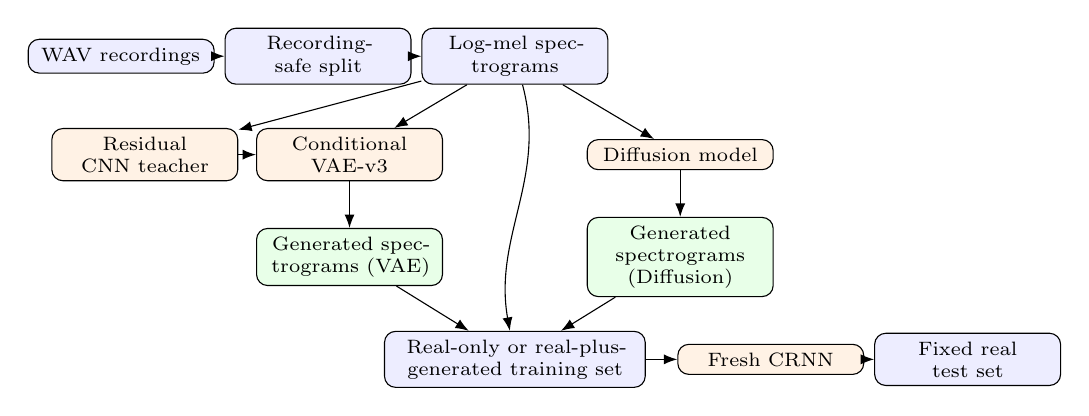
\begin{tikzpicture}[
    block/.style={draw,rounded corners,align=center,inner sep=3pt,
                  text width=2.15cm,font=\scriptsize},
    data/.style={block,fill=blue!7},
    model/.style={block,fill=orange!10},
    generated/.style={block,fill=green!9},
    arrow/.style={-{Latex[length=1.7mm]},thin}
  ]
    \node[data] (wav) at (-5.0,0) {WAV recordings};
    \node[data] (split) at (-2.5,0) {Recording-safe split};
    \node[data] (mel) at (0,0) {Log-mel spectrograms};
    \node[model] (teacher) at (-4.7,-1.25) {Residual CNN teacher};
    \node[model] (vae) at (-2.1,-1.25) {Conditional VAE-v3};
    \node[model] (diff) at (2.1,-1.25) {Diffusion model};
    \node[generated] (gvae) at (-2.1,-2.55) {Generated spectrograms (VAE)};
    \node[generated] (gdiff) at (2.1,-2.55) {Generated spectrograms (Diffusion)};
    \node[data,text width=3.1cm] (train) at (0,-3.85)
      {Real-only or real-plus-generated training set};
    \node[model] (crnn) at (3.25,-3.85) {Fresh CRNN};
    \node[data] (test) at (5.75,-3.85) {Fixed real test set};
    \draw[arrow] (wav) -- (split);
    \draw[arrow] (split) -- (mel);
    \draw[arrow] (mel) -- (teacher);
    \draw[arrow] (mel) -- (vae);
    \draw[arrow] (teacher) -- (vae);
    \draw[arrow] (mel) -- (diff);
    \draw[arrow] (vae) -- (gvae);
    \draw[arrow] (diff) -- (gdiff);
    \draw[arrow] (gvae) -- (train);
    \draw[arrow] (gdiff) -- (train);
    \draw[arrow] (mel) to[out=-75,in=100] (train);
    \draw[arrow] (train) -- (crnn);
    \draw[arrow] (crnn) -- (test);
  \end{tikzpicture}}
  \caption{BirdGEN pipeline. Both generated-spectrogram branches feed the same
  downstream-classifier protocol.}
  \label{fig:pipeline}
\end{figure}

\subsection{Classifiers}

The 1.66-M-parameter Residual CNN uses six residual blocks and global
average/max pooling. It is retained as an architecture-comparison reference,
and its frozen features and logits guide VAE-v3 training. It does not score or
compare VAE and Diffusion in the maintained independent evaluation. The selected
404-k-parameter CRNN combines
convolutional spectral features with a bidirectional GRU and temporal pooling
\cite{cakir2017crnn}. An independent frozen CRNN supplies generation-quality
diagnostics, while freshly initialized CRNNs provide the downstream
augmentation evidence.

\subsection{Conditional VAE Evolution}

We selected a conditional VAE (CVAE) rather than an unconditional VAE, because 
every training spectrogram is paired with a bird-species label, and the
downstream task requires controllable, class-labelled augmentation
\cite{kingma2014aevb,sohn2015cvae}. The species label $y$ conditions both the
encoder $q_\phi(z\mid x,y)$ and decoder $p_\theta(x\mid z,y)$. Since the
requested class is supplied explicitly, the latent variables do not need to
represent species identity alone and can thus focus more on within-species variation,
such as vocalization type, pitch, and timing. Conditioning reduces
cross-species ambiguity, although it does not by itself guarantee realistic or
diverse outputs.

V1 established a CVAE baseline with a 128-dimensional global latent vector, species
embeddings concatenated at the encoder and decoder, and MSE+KL loss. Its
compressed bottleneck and pixel-level reconstruction objective tended to smooth
narrow calls, pitch tracks, and transient structure. V2 replaced the global
vector with a $16\times8\times8$ spatial latent and added residual FiLM
conditioning \cite{perez2018film}, resize-convolution, and event-weighted,
multiscale, and time/frequency-gradient reconstruction losses. These changes
were intended to preserve the locations and edges of short transients and
harmonics. For generation, V2 fitted one moment-matched diagonal Gaussian to
the training posteriors of each species. Although this reduced the mismatch
with standard-normal sampling, a single Gaussian could still average distinct
vocalization modes within a species.

V3 increased the latent resolution to $16\times16\times16$, used a lower KL
weight with a longer warmup and per-channel free bits to reduce excessive
latent compression and help retain information needed for fine
spectro-temporal detail. It also added feature and label consistency losses
from a frozen, supervised Residual CNN species classifier trained on labeled
real spectrograms, providing species-aware guidance. For generation, V3 replaced each
single species-level Gaussian with a train-only posterior-anchor bank, allowing
samples to be drawn near multiple encoded vocalization examples. This
generation-time strategy mitigates the practical mismatch between the
standard-normal prior and learned posteriors, but it does not replace the prior
used to train the checkpoint. Since multiple components were modified between versions, 
the results show the improvement of each complete model rather than the individual causal
effect of any single modification.

VAE-v3 has approximately 5.37~M parameters. Species embeddings modulate
residual encoder and decoder blocks through FiLM. Its training objective is
\begin{equation}
\mathcal{L}
=
\mathcal{L}_{\mathrm{event}}
+0.25\mathcal{L}_{\mathrm{ms}}
+0.60\left(
    \mathcal{L}_{\Delta t}
    +\mathcal{L}_{\Delta f}
\right)
+\beta\mathcal{L}_{\mathrm{KL,free}}
+s_{\mathrm{cls}}
\left[
    0.08\mathcal{L}_{\mathrm{feat}}
    +0.03\mathcal{L}_{\mathrm{label}}
\right].
\label{eq:vae-loss}
\end{equation}
Here, $\mathcal{L}_{\mathrm{event}}$ is an event-weighted L1 reconstruction
term, $\mathcal{L}_{\mathrm{ms}}$ averages L1 losses at multiple resolutions,
and $\mathcal{L}_{\Delta t}$ and $\mathcal{L}_{\Delta f}$ are edge-weighted L1
discrepancies between first-order time and frequency differences. The KL
coefficient $\beta$ is warmed up to
$5\times10^{-4}$ over 20 epochs, while $s_{\mathrm{cls}}$ increases to one
over eight epochs. The free-bits term applies a 0.25-nat floor to the
batch-and-spatial mean KL of each latent channel, so reducing a channel's KL
below this threshold provides no further optimization benefit. Multiscale and
feature-space terms are motivated by
\cite{mathieu2016multiscale,johnson2016perceptual}, and free bits follow
\cite{kingma2016iaf}.

For a training anchor $i$ with the requested species label, the encoder defines
a diagonal-Gaussian posterior
$q_\phi(z\mid x_i,y)=
\mathcal{N}(\mu_i,\operatorname{diag}(\sigma_i^2))$.
The corrected generation-time sampler applies temperature only to its
stochastic residual:
\begin{equation}
z = \mu_i+T\sigma_i\odot\epsilon,
\qquad
T=0.35,\quad \epsilon\sim\mathcal{N}(0,I).
\label{eq:vae-anchor-sampling}
\end{equation}
This correction affects post-training sampling only; the training-time
reparameterization and VAE checkpoint were unchanged. The train-only,
content-safe posterior bank retained 256 Northern Cardinal, 247 Song Sparrow,
and 256 American Robin anchors, and the three generation-seed VAE pools were
regenerated from this bank. The method is conceptually related to
mixture-of-posteriors priors such as VampPrior \cite{tomczak2018vampprior},
but uses fixed encoded training examples rather than learned pseudo-inputs and
does not modify the training objective. 

\subsection{Diffusion Model}
% Intentionally left blank for Vincent Wang's canonical Diffusion method and citations.

\section{Experimental Methodology}

Classifier architectures were selected on validation data across seeds 42,
123, and 777, then evaluated on held-out test recordings. VAE evidence is
separated into paired deterministic reconstruction, unpaired generated-sample
quality, and downstream classifier utility. To address the presentation
feedback, each frozen generated sample was compared with its nearest
same-species test spectrogram in the standardized-logmel domain, with a
leave-one-out real-test reference. The test set was used only for this final
evaluation; low MSE can also indicate copying or limited diversity.

For the primary experiment, each fresh CRNN sees 50 real examples per species.
Three real-subset seeds crossed with three classifier seeds give nine matched
blocks. Every block evaluates $50+0$, $50+50$, $50+100$, and $50+200$
real-plus-generated samples per species, separately for VAE and Diffusion.
Ratios are selected using the 510-row generator-safe validation subset; only
the shared $50+0$ baseline and each generator's selected ratio reach the fixed
489-row real test set. Architecture,
augmentation, and optimizer-step budget are matched. No existing pretrained
classifier is augmented, and the Residual CNN is not a generated-sample
evaluator. The recorded runtime benchmark timed five fresh in-memory
600-spectrogram repeats per model on the same GPU, precision, and batch size
after warm-up. CUDA was synchronized around generator sampling through the
final normalized tensor; model loading, existing arrays, file output,
plotting, and metric computation were excluded. Models were measured
sequentially: the completed Diffusion benchmark was retained and VAE-v3 was
remeasured with the filtered bank, with no Diffusion sampling rerun.

\section{Experimental Results}

\paragraph{Classifier selection.}
Among the four evaluated classifier architectures, the 404-k-parameter CRNN
achieved the highest controlled three-seed validation macro-F1
($90.45\%\pm1.45\%$). The validation-selected seed-777 checkpoint subsequently
obtained 89.98\% accuracy and 90.16\% macro-F1 on the 489-clip held-out real
test set.

\paragraph{VAE diagnostics.}
The recorded test-set reconstruction MSE in the globally standardized log-mel domain was
0.1533 for V1, 0.0654 for V2, and 0.0281 for V3. V2 and V3 used deterministic
posterior-mean reconstructions, whereas the historical V1 evaluation sampled
from its posterior; the trend is therefore descriptive rather than a strictly
matched deterministic comparison. V3 test MAE was 0.1261 and spectral
convergence was 0.1794. MSE is an evaluation diagnostic rather than V3's
complete training objective, and these input-to-reconstruction values are not
generated-to-real distances.

\begin{figure}[t]
  \centering
  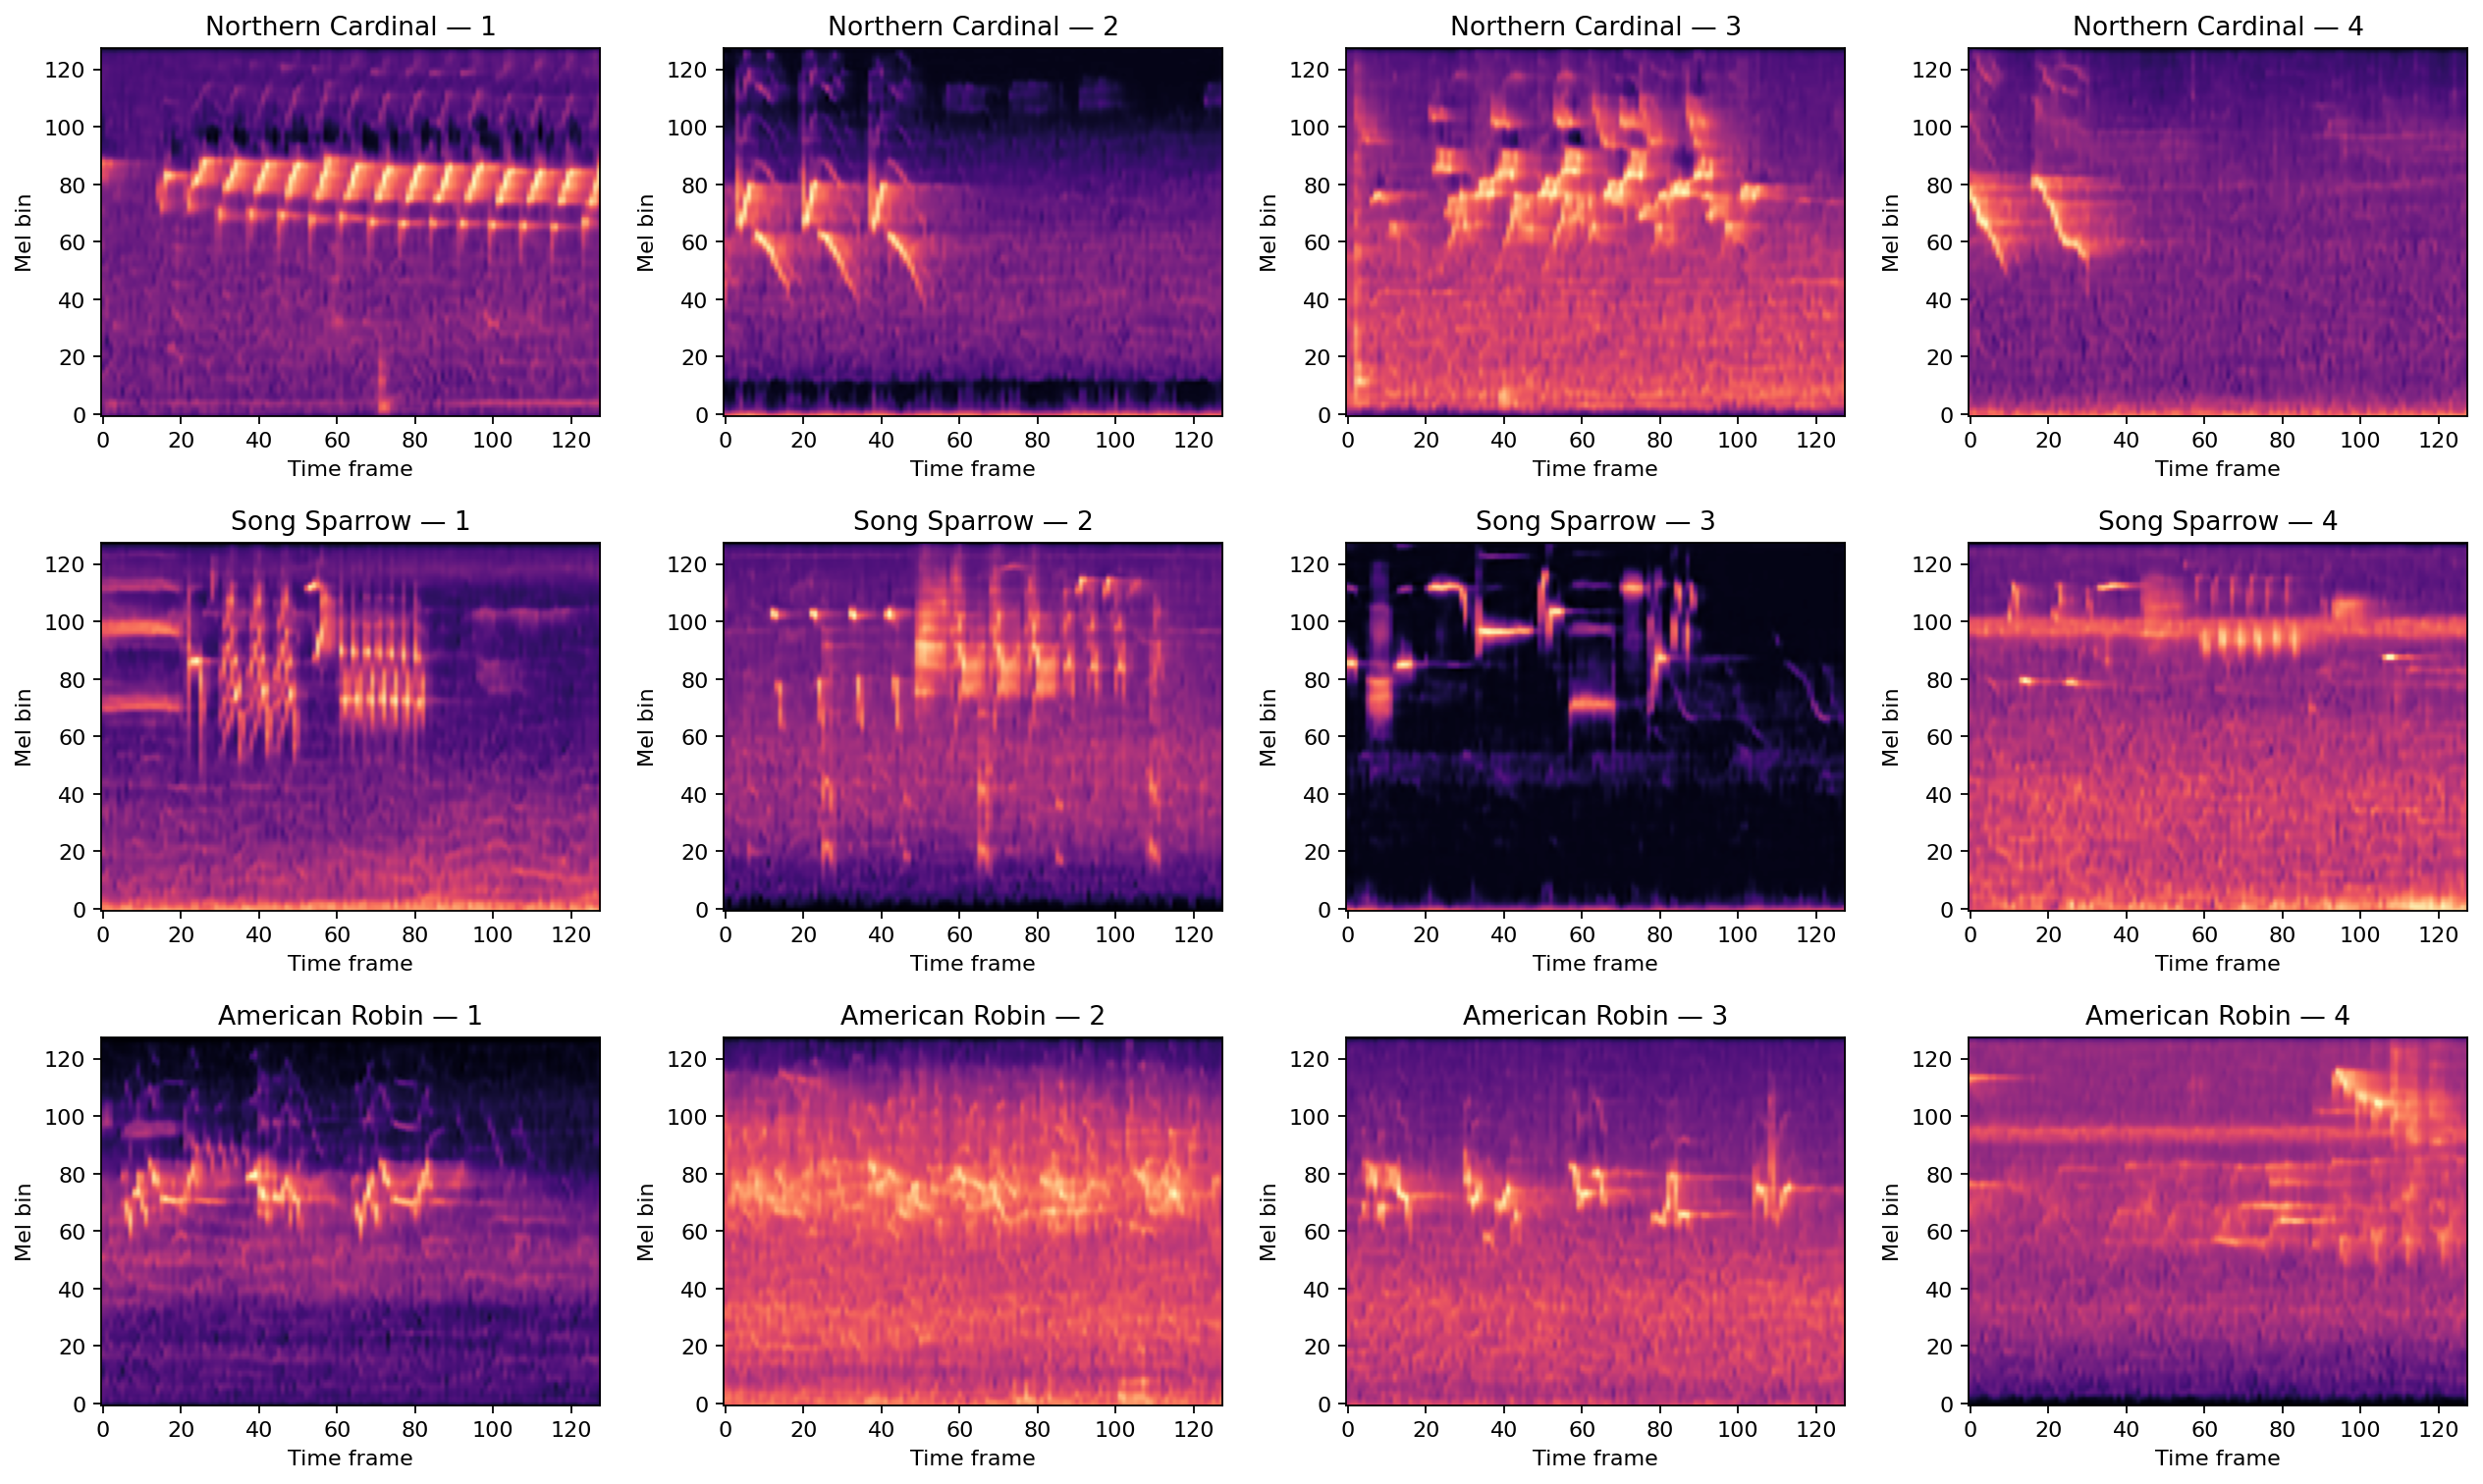
\includegraphics[width=\linewidth]{../../reports/vae/conditional_vae_v3/conditional_samples.png}
  \caption{Existing VAE-v3 notebook posterior-anchor samples at temperature
  0.35: four examples per species (48 samples were saved in total). Panels are
  independently color-normalized; spectrogram appearance alone does not
  establish waveform realism.}
  \label{fig:vae-samples}
\end{figure}

For the separately verified seed-42 notebook pool (16 samples/species), the
mean same-species generated-to-test nearest-neighbor pixel MSE was 0.5120
(SD 0.1998; median 0.4501; IQR 0.3878--0.6231); the leave-one-out real-to-real
reference mean was 0.3350 (SD 0.1419; median 0.3185; IQR 0.2368--0.4154).
The generated-to-test/real-to-real means by species were 0.4308/0.3237 for
American Robin, 0.5579/0.3650 for Northern Cardinal, and 0.5474/0.3175 for
Song Sparrow. These unpaired pixel-space summaries use 48 and 489 queries,
respectively, and nearest-neighbor MSE can reward copying; they are neither
perceptual-realism nor waveform-quality scores. This hash-recorded diagnostic
used a separately reconstructed notebook pool (temperature 0.35; train-only
posterior bank), rather than the canonical pools used downstream. Although
both use standardized log-mels, 0.5120 and 0.0281 are not comparable because
they summarize generated-to-nearest-test and input-to-own-reconstruction
pairs, respectively. The Residual CNN remains a frozen VAE training teacher
and supplies no independent VAE--Diffusion evaluation.
Table~\ref{tab:quality} reports the current audited pools using the selected
CRNN and its shared feature space. Values are three-generation-seed means; the
feature rows additionally average the three species.

\begin{table}[t]
  \caption{Frozen selected-CRNN and feature-space generated-sample diagnostics.}
  \label{tab:quality}
  \centering
  \small
  \resizebox{\linewidth}{!}{%
  \begin{tabular}{@{}lll@{}}
    \toprule
    Metric & VAE-v3 & Diffusion \\
    \midrule
    Target-label accuracy / CRNN macro-F1 & 96.67\% / 96.66\% & 92.44\% / 92.42\% \\
    Classifier-feature Fr\'echet distance & 22.8950 & 41.2550 \\
    Feature precision / feature recall & 0.8528 / 0.8972 & 0.5654 / 0.8207 \\
    Feature density / coverage / diversity ratio & 0.6423 / 0.7419 / 0.8719 & 0.3114 / 0.4845 / 1.0083 \\
    Pixel Wasserstein / near-train fraction / exact copies & 0.0787 / 36.67\% / 0 & 0.1916 / 2.50\% / 0 \\
    \bottomrule
  \end{tabular}}
\end{table}

\paragraph{Low-resource augmentation.}
\begin{table}[t]
  \caption{Completed low-resource CRNN study across nine matched blocks.}
  \label{tab:low-resource}
  \centering
  \small
  \begin{tabular}{@{}lll@{}}
    \toprule
    Per-species condition & Val. macro-F1 (VAE / Diff.) & Test status \\
    \midrule
    $50+0$ & Shared real-only reference & Evaluated baseline \\
    $50+50$ & 84.53\% / 85.45\% & Not selected \\
    $50+100$ & 85.88\% / 86.06\% & Not selected \\
    $50+200$ & 86.47\% / 86.84\% & Selected for both \\
    \bottomrule
  \end{tabular}
\end{table}

Test reporting is limited to the shared $50+0$ baseline and the independently
selected $+200$ condition. Mean held-out macro-F1 was 84.75\% for real-only,
87.48\% for VAE-v3, and 86.21\% for Diffusion. The paired changes were
$+2.72$ percentage points for VAE-v3 (7/9 positive blocks; descriptive
block-bootstrap interval $+1.00$ to $+4.65$) and $+1.46$ points for Diffusion
(6/9; $+0.15$ to $+2.89$).

\paragraph{Equal-count generator timing.}
The recorded benchmark generated 600 fresh in-memory spectrograms (200 per
species) per synchronized repeat after warm-up. The package retains every
repeat's seconds, throughput, peak accelerator memory, hardware, precision,
batch size, sampler settings, seed, measurement sequence, and timing boundary.
Pre-existing arrays are not timing evidence.
\begin{table}[t]
  \caption{Generator-only timing comparison for matched fresh outputs.}
  \label{tab:timing}
  \centering
  \small
  \resizebox{\linewidth}{!}{%
  \begin{tabular}{@{}lrrrr@{}}
    \toprule
    Model & Outputs/repeat & Repeat seconds & Samples/s & Peak accelerator memory \\
    \midrule
    VAE-v3 (corrected sampler) & 600 & $0.3058\pm0.0096$ & 1963.276 & 0.185 GiB \\
    Diffusion (100-step DDIM) & 600 & $412.3090\pm2.8120$ & 1.455 & 0.333 GiB \\
    Difference / Diffusion-to-VAE ratio & 600 & 412.0032 / $1348.09\times$ & -- & -- \\
    \bottomrule
  \end{tabular}}
\end{table}
The median [Q1, Q3] repeat time was 0.3046 [0.2983, 0.3076] seconds for VAE-v3
and 411.1814 [410.9396, 411.2319] seconds for Diffusion. These measurements use
FP32, batch size 8, five warm-up batches, five CUDA-synchronized repeats, and an
RTX 4070 SUPER. They exclude loading, conversion, transfer, file I/O, and audio
decoding. The completed Diffusion benchmark was retained; VAE-v3 was
remeasured afterward using the filtered 759-anchor bank, and no Diffusion
sampling was rerun.

\section{Discussion}

In the simulated low-resource setting, both validation-selected $+200$ arms
improved mean held-out macro-F1 versus their matched real-only controls. The
nine blocks reuse overlapping real subsets, so the intervals are descriptive
and the largest tested ratio is not an estimated optimum. This result applies
to newly initialized low-resource CRNNs, not the historical full-data CRNN.
Reconstruction MSE rewards pixel proximity, the Residual CNN is coupled to
V3 training and therefore restricted to its teacher role, and a closed-set
independent CRNN cannot reject unknown or noisy inputs. Spectrogram and
classifier metrics also do not replace listening or waveform-level evaluation
\cite{bhatia2022birdsong}. VAE-v3 has higher CRNN target
compatibility, lower macro-species Fr\'echet distance, and higher feature
precision/coverage in these pools, but it also has a much larger near-training
feature fraction. Diffusion has a diversity ratio nearer one and lower
copy-risk flags. Separately, Diffusion took $1348.09\times$ the VAE-v3
generator time under the recorded boundary.

\section{Conclusion}

BirdGEN now has corrected three-seed generator evidence, a completed matched
low-resource CRNN study, and a matched timing comparison. Validation selected
$+200$/species for both models; the mean paired macro-F1 changes were $+2.72$
points for VAE-v3 and $+1.46$ points for Diffusion. Quality diagnostics remain
metric-specific rather than a composite winner, and the efficiency result is
limited to generator-only spectrogram sampling on the recorded hardware.

\clearpage
\begin{thebibliography}{99}
\small

\bibitem{kahl2021birdnet}
S. Kahl, C. M. Wood, M. Eibl, and H. Klinck,
``BirdNET: A deep learning solution for avian diversity monitoring,''
\emph{Ecological Informatics}, vol. 61, Art. no. 101236, 2021.

\bibitem{guei2024ecogen}
A.-C. Guei, S. Christin, N. Lecomte, and E. Hervet,
``ECOGEN: Bird sounds generation using deep learning,''
\emph{Methods in Ecology and Evolution}, vol. 15, pp. 69--79, 2024.

\bibitem{kingma2014aevb}
D. P. Kingma and M. Welling, ``Auto-Encoding Variational Bayes,'' in
\emph{Proc. Int. Conf. Learn. Represent. (ICLR)}, 2014.

\bibitem{sohn2015cvae}
K. Sohn, H. Lee, and X. Yan, ``Learning structured output representation using
deep conditional generative models,'' in \emph{Adv. Neural Inf. Process.
Syst.}, vol. 28, pp. 3483--3491, 2015.

\bibitem{shanbhagBirdSongDataset}
V. Shanbhag, ``Bird song data set,'' Kaggle, ver. 1. [Online]. Available:
\url{https://www.kaggle.com/datasets/vinayshanbhag/bird-song-data-set}.
[Accessed: Aug. 13, 2026].

\bibitem{cakir2017crnn}
E. Cakir, G. Parascandolo, T. Heittola, H. Huttunen, and T. Virtanen,
``Convolutional recurrent neural networks for polyphonic sound event
detection,'' \emph{IEEE/ACM Trans. Audio, Speech, Lang. Process.}, vol. 25,
no. 6, pp. 1291--1303, 2017.

\bibitem{perez2018film}
E. Perez, F. Strub, H. de Vries, V. Dumoulin, and A. Courville, ``FiLM: Visual
reasoning with a general conditioning layer,'' in \emph{Proc. AAAI Conf.
Artif. Intell.}, vol. 32, no. 1, pp. 3942--3951, 2018.

\bibitem{mathieu2016multiscale}
M. Mathieu, C. Couprie, and Y. LeCun, ``Deep multi-scale video prediction
beyond mean square error,'' in \emph{Proc. ICLR}, 2016.

\bibitem{johnson2016perceptual}
J. Johnson, A. Alahi, and L. Fei-Fei, ``Perceptual losses for real-time style
transfer and super-resolution,'' in \emph{Computer Vision--ECCV}, pp.
694--711, 2016.

\bibitem{kingma2016iaf}
D. P. Kingma, T. Salimans, R. Jozefowicz, X. Chen, I. Sutskever, and M.
Welling, ``Improved variational inference with inverse autoregressive flow,''
in \emph{Adv. Neural Inf. Process. Syst.}, vol. 29, pp. 4743--4751, 2016.

\bibitem{tomczak2018vampprior}
J. Tomczak and M. Welling, ``VAE with a VampPrior,'' in \emph{Proc. AISTATS},
PMLR, vol. 84, pp. 1214--1223, 2018.

\bibitem{bhatia2022birdsong}
R. R. Bhatia and T. H. Kinnunen, ``An initial study on birdsong re-synthesis
using neural vocoders,'' in \emph{Speech and Computer}, pp. 64--74, 2022.

\end{thebibliography}

\clearpage
\appendix
\section{Supplementary Reproducibility Notes}

VAE-v3 used AdamW with learning rate $2\times10^{-4}$, batch size 24, a
20-epoch KL warm-up, and checkpoint selection by the complete validation
objective. The portable pool generator now applies the notebook's sampling
temperature 0.35 explicitly. The VAE checkpoint was not retrained. The
existing posterior bank was filtered to 256 Northern Cardinal, 247 Song
Sparrow, and 256 American Robin anchors, and the three canonical VAE pools
were regenerated with the corrected sampler.
The reported generated-to-test MSE instead uses a separate, hash-recorded
seed-42 pool reconstructed with the original notebook, 16 samples per species,
and the train-only posterior bank. This MSE package remains separate from the
three-seed augmentation pools and does not replace their quality or downstream
CRNN evidence.

For the equal-count timing study, each model generated 600 spectrograms
(200 per species) in FP32 with batch size 8 on the same hardware. Five warm-up
batches preceded five synchronized repeats. Models were measured sequentially,
not interleaved: the completed Diffusion benchmark was retained and VAE-v3 was
remeasured after the bank filter. The sole timing boundary is generator
sampling through the final normalized spectrogram tensor; model loading,
existing arrays, file output, plotting, and metric computation are excluded.
The package preserves repeat seconds, throughput, peak accelerator memory,
hardware, precision, batch size, seeds, sampler settings, and the
timing-boundary description.

\end{document}
